\documentclass[aspectratio=169]{beamer}
\usetheme{Madrid}
\usecolortheme{seahorse}
\usepackage{amsmath,amssymb}
\usepackage{tikz}
\usepackage{booktabs}
\usepackage{multirow}
\usetikzlibrary{shapes.geometric,arrows.meta,positioning,fit,backgrounds}

\newcommand{\N}{\mathcal{N}}
\DeclareMathOperator*{\argmin}{arg\,min}

\setbeamertemplate{navigation symbols}{}
\setbeamertemplate{footline}[frame number]

\title[Fragmentation-Aware GPU Scheduling]{Fragmentation-Aware GPU Cluster Scheduling}
\subtitle{A Statistically-Grounded Benchmark, an Improved Algorithm,\\ and an Honest Account of What It Does and Does Not Fix}
\author{Thesis Defense}
\institute{gputrace + py\_sim}
\date{\today}

\begin{document}

% =====================================================================
\begin{frame}
\titlepage
\end{frame}

% =====================================================================
\begin{frame}{The Problem, In One Picture}
\centering
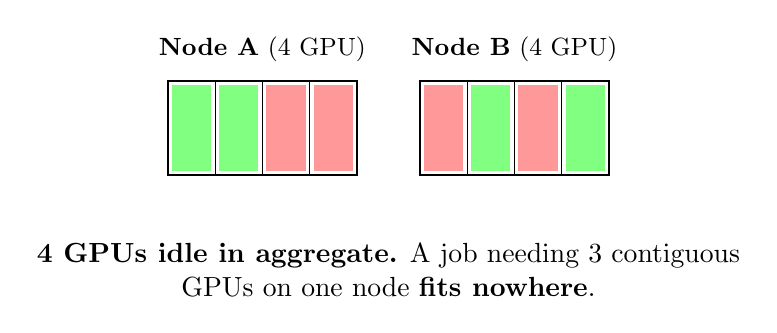
\begin{tikzpicture}[scale=1.0, every node/.style={font=\small}]
  \draw[thick] (0,0) rectangle (2.4,1.2);
  \node at (1.2,1.6) {\textbf{Node A} (4 GPU)};
  \foreach \i/\c in {0/green!50,1/green!50,2/red!40,3/red!40} {
    \draw (\i*0.6,0) rectangle (\i*0.6+0.6,1.2);
    \fill[\c] (\i*0.6+0.05,0.05) rectangle (\i*0.6+0.55,1.15);
  }
  \draw[thick] (3.2,0) rectangle (5.6,1.2);
  \node at (4.4,1.6) {\textbf{Node B} (4 GPU)};
  \foreach \i/\c in {0/red!40,1/green!50,2/red!40,3/green!50} {
    \draw (3.2+\i*0.6,0) rectangle (3.2+\i*0.6+0.6,1.2);
    \fill[\c] (3.2+\i*0.6+0.05,0.05) rectangle (3.2+\i*0.6+0.55,1.15);
  }
  \node[align=center, font=\normalsize] at (2.8,-1.2)
    {\textbf{4 GPUs idle in aggregate.} A job needing 3 contiguous\\
     GPUs on one node \textbf{fits nowhere}.};
\end{tikzpicture}

\vspace{0.6cm}
\begin{center}
\alert{Utilization dashboards say 50\% free. Usable free capacity is 0.}
\end{center}
\end{frame}

% =====================================================================
\begin{frame}{This Is a Real, Costly, Recent Problem}
\begin{itemize}
  \item GPU-sharing (multiple jobs per physical GPU) is now standard practice
  \item Fragmentation Gradient Descent (FGD, USENIX ATC~'23) was the first
    scheduler to treat this as a first-class objective
  \item \textbf{FGD is only three years old} -- this is a genuinely young
    research niche, with a lot still unexplored
  \item Cloud infrastructure keeps finding new ways to fail under resource
    contention: a 15-hour, 60-country AWS outage in October 2025 traced to
    a cascading resource issue; a Google auth outage the same year fixed
    only by \emph{adding capacity}
\end{itemize}
\vspace{0.4cm}
\begin{alertblock}{The gap this thesis targets}
Every public evaluation of FGD-lineage schedulers we found replays
\textbf{one fixed historical trace}. A fixed recording cannot contain
events that had not yet happened when it was collected.
\end{alertblock}
\end{frame}

% =====================================================================
\begin{frame}{Thesis Statement}
\begin{enumerate}
  \item[\textbf{1.}] A synthetic, statistically-grounded, multi-scenario
    benchmark is \textbf{necessary} to evaluate fragmentation-aware
    scheduling honestly -- a single trace structurally cannot contain the
    failure modes that matter most.
  \vspace{0.3cm}
  \item[\textbf{2.}] FGD's own fragmentation metric has \textbf{two
    specific, checkable weaknesses} that can be fixed -- producing a real,
    statistically significant improvement over FGD specifically, while
    \textbf{honestly not} claiming a new state of the art against every
    alternative.
\end{enumerate}
\end{frame}

% =====================================================================
\section{Literature \& Research Gap}
\begin{frame}{From Bin Packing to GPU Scheduling}
\centering
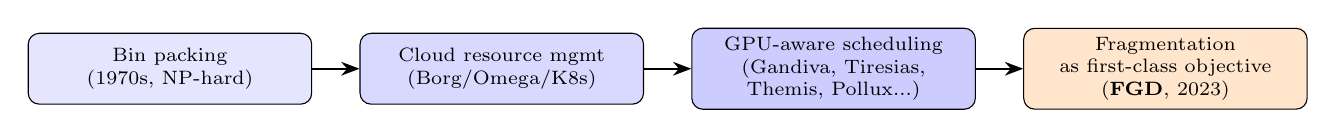
\begin{tikzpicture}[
  node distance=0.4cm and 0.6cm,
  box/.style={draw, rounded corners, minimum width=3.6cm, minimum height=0.9cm, align=center, font=\scriptsize},
  arr/.style={-{Stealth}, thick}
]
  \node[box, fill=blue!10] (bp) {Bin packing\\(1970s, NP-hard)};
  \node[box, right=of bp, fill=blue!15] (crm) {Cloud resource mgmt\\(Borg/Omega/K8s)};
  \node[box, right=of crm, fill=blue!20] (gpu) {GPU-aware scheduling\\(Gandiva, Tiresias,\\Themis, Pollux...)};
  \node[box, right=of gpu, fill=orange!20] (frag) {Fragmentation\\as first-class objective\\(\textbf{FGD}, 2023)};
  \draw[arr] (bp) -- (crm);
  \draw[arr] (crm) -- (gpu);
  \draw[arr] (gpu) -- (frag);
\end{tikzpicture}

\vspace{0.5cm}
\begin{block}{The twist}
None of the six major GPU-scheduling systems before FGD treats
\emph{where, geometrically,} a job lands as its primary objective --
placement quality was always a side effect of some other goal.
\end{block}
\end{frame}

\begin{frame}{Two Research Gaps}
\begin{columns}
\column{0.48\textwidth}
\textbf{Gap 1: The metric itself}
\begin{itemize}
  \item FGD's 5 representative shapes are weighted \textbf{uniformly}
  \item Each shape's coordinates are \textbf{per-dimension quantiles} --
    can be a ``chimera'' matching no real job
\end{itemize}
\column{0.48\textwidth}
\textbf{Gap 2: The evaluation}
\begin{itemize}
  \item Every FGD-lineage paper evaluates on \textbf{one fixed trace}
  \item Real traces are non-stationary (Google, Azure trace studies) --
    a fixed slice is one draw, not the distribution
\end{itemize}
\end{columns}
\vspace{0.5cm}
\centering
\textbf{This thesis addresses both.}
\end{frame}

% =====================================================================
\section{System Architecture}
\begin{frame}{Simulator Lineage: Why We Rebuilt in Python}
\centering
\resizebox{0.9\textwidth}{!}{%
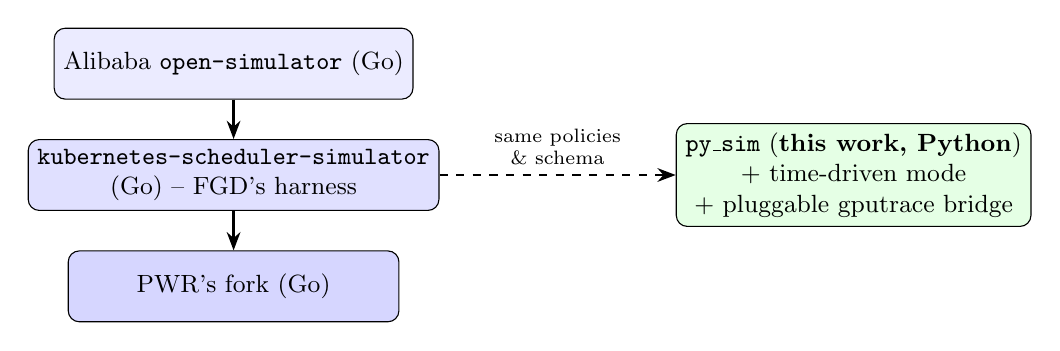
\begin{tikzpicture}[
  node distance=0.5cm and 1.2cm,
  box/.style={draw, rounded corners, minimum width=4.2cm, minimum height=0.9cm, align=center, font=\small},
  arr/.style={-{Stealth}, thick}
]
  \node[box, fill=blue!8] (sim0) {Alibaba \texttt{open-simulator} (Go)};
  \node[box, below=of sim0, fill=blue!12] (sim1) {\texttt{kubernetes-scheduler-simulator}\\(Go) -- FGD's harness};
  \node[box, below=of sim1, fill=blue!16] (sim2) {PWR's fork (Go)};
  \node[box, right=3.0cm of sim1, fill=green!10] (ours) {\texttt{py\_sim} (\textbf{this work, Python})\\+ time-driven mode\\+ pluggable gputrace bridge};
  \draw[arr] (sim0) -- (sim1);
  \draw[arr] (sim1) -- (sim2);
  \draw[arr, dashed] (sim1) -- node[above,font=\scriptsize,align=center]{same policies\\\& schema} (ours);
\end{tikzpicture}%
}
\vspace{0.4cm}
\begin{itemize}
  \item Reimplemented (not forked): first-class Python statistical tooling
  \item Added a \textbf{time-driven} evaluation mode -- several stress
    scenarios are defined entirely by \emph{timing} and invisible to
    static-mode evaluation alone
\end{itemize}
\end{frame}

\begin{frame}{gputrace: A Pluggable Stress-Test Generator}
\centering
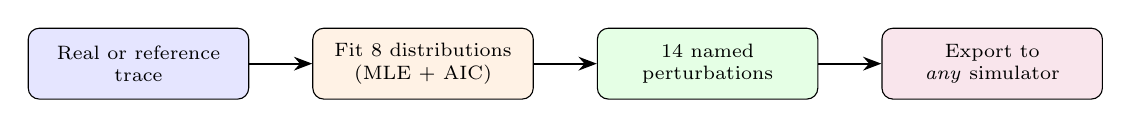
\begin{tikzpicture}[
  node distance=0.4cm and 0.8cm,
  box/.style={draw, rounded corners, minimum width=2.8cm, minimum height=0.9cm, align=center, font=\scriptsize},
  arr/.style={-{Stealth}, thick}
]
  \node[box, fill=blue!10] (loader) {Real or reference\\trace};
  \node[box, right=of loader, fill=orange!10] (fit) {Fit 8 distributions\\(MLE + AIC)};
  \node[box, right=of fit, fill=green!10] (gen) {14 named\\perturbations};
  \node[box, right=of gen, fill=purple!10] (export) {Export to\\\emph{any} simulator};
  \draw[arr] (loader) -- (fit);
  \draw[arr] (fit) -- (gen);
  \draw[arr] (gen) -- (export);
\end{tikzpicture}

\vspace{0.5cm}
\begin{exampleblock}{Each scenario perturbs one named, specific mechanism}
bursty arrivals \textbullet\ GPU-type contention \textbullet\ spot-preemption
churn \textbullet\ LLM-inference bursts \textbullet\ MoE expert skew
\textbullet\ checkpoint I/O storms \textbullet\ 9 more
\end{exampleblock}
\end{frame}

% =====================================================================
\section{Our Contribution}
\begin{frame}{Two Checkable Weaknesses in FGD}
\[
  U(n,t)=\frac{1}{|\hat P|}\sum_{\hat p\in\hat P}\mathbb{1}[\neg\mathrm{fits}(\hat p,n,t)]
\]
\begin{columns}
\column{0.5\textwidth}
\textbf{Weakness 1: Uniform weighting}\\
\small All 5 shapes weighted equally, though they represent unequal
population mass (10th vs.\ 50th percentile).
\column{0.5\textwidth}
\textbf{Weakness 2: Chimera shapes}\\
\small Each shape's cpu/gpu/gpu-count are \emph{independent} marginal
quantiles -- may match no real job.
\end{columns}
\vspace{0.4cm}
\begin{alertblock}{Both are provable from FGD's own definition -- not assumptions about intent.}
\end{alertblock}
\end{frame}

\begin{frame}{w-fgd and w-fgd-balanced}
\textbf{Fix:} stratify jobs by demand magnitude, take each stratum's
\emph{medoid} (a real job) weighted by population share:
\[
  \hat p_k=\argmin_{p\in S_k}|m(p)-\mathrm{median}(m(S_k))|, \qquad w_k=\frac{|S_k|}{|P|}
\]
\[
  \pi_{\text{w\_fgd}}(p,t)=\argmin_{n}\big[U_w(n,t{\oplus}p)-U_w(n,t)\big]
\]
\textbf{w-fgd-balanced} adds slack-preservation regularization:
\[
  \pi_{\text{w\_fgd\_bal}}(p,t)=\argmin_{n}\Big[U_w(n,t{\oplus}p)-U_w(n,t) + \lambda\,\phi^{\text{gpu}}(n,t{\oplus}p)\Big]
\]
\centering\small $\lambda=0$ recovers w-fgd exactly (verified by unit test)
\end{frame}

% =====================================================================
\section{Results}
\begin{frame}{Did We Break FGD? Yes -- Specifically}
\centering
\begin{tabular}{lrrr}
\toprule
metric (mode) & fgd & w\_fgd\_balanced & Wilcoxon $p$ \\
\midrule
rejection rate (static) & 0.3352 & 0.3133 & \textbf{0.0035} \\
SLA violation (time-driven) & 0.1206 & 0.1022 & \textbf{0.0365} \\
p95 wait time & 326.1s & 344.1s & 0.507 (n.s.) \\
fairness (Jain) & 0.1902 & 0.1805 & 0.196 (n.s.) \\
\bottomrule
\end{tabular}
\vspace{0.5cm}
\begin{alertblock}{But, reported honestly}
Statistically \textbf{indistinguishable} from the simplest existing
baseline, \texttt{least\_requested} ($p=0.81$).
\end{alertblock}
\end{frame}

\begin{frame}{Full Ranking, All 13 Algorithms}
\centering
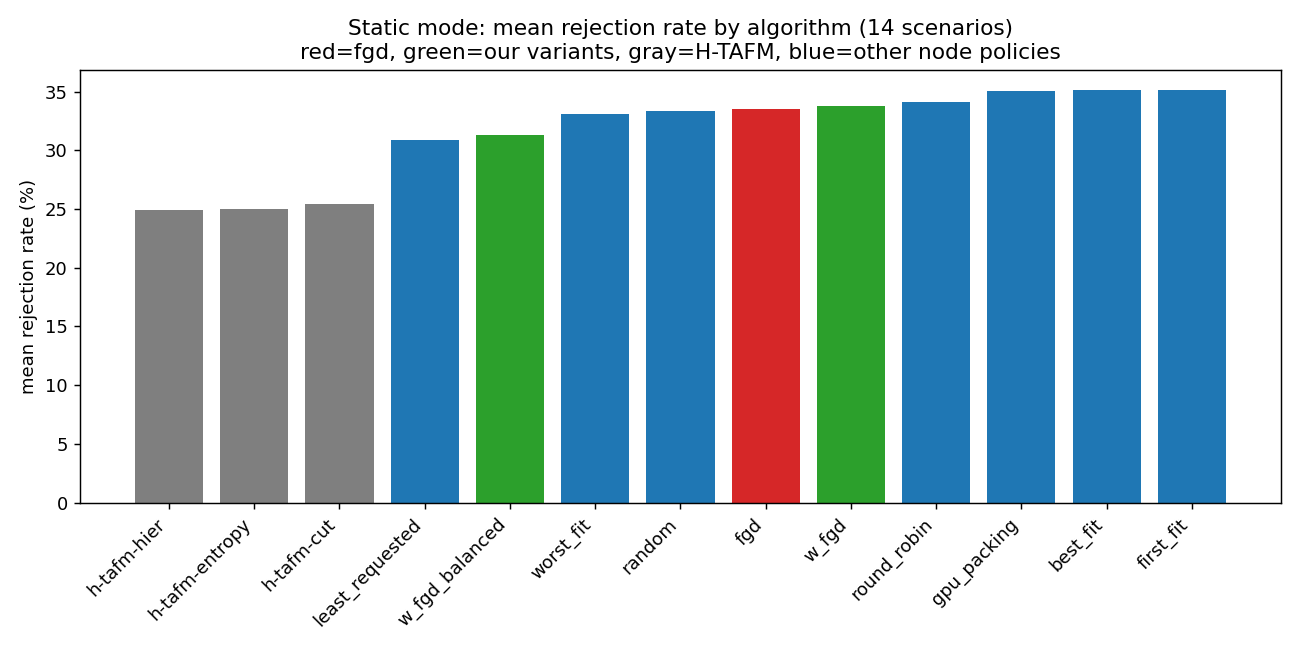
\includegraphics[width=0.85\textwidth]{plots/01_static_rejection_by_algorithm.png}
\end{frame}

\begin{frame}{fgd vs.\ w\_fgd vs.\ w\_fgd\_balanced, Per Scenario}
\centering
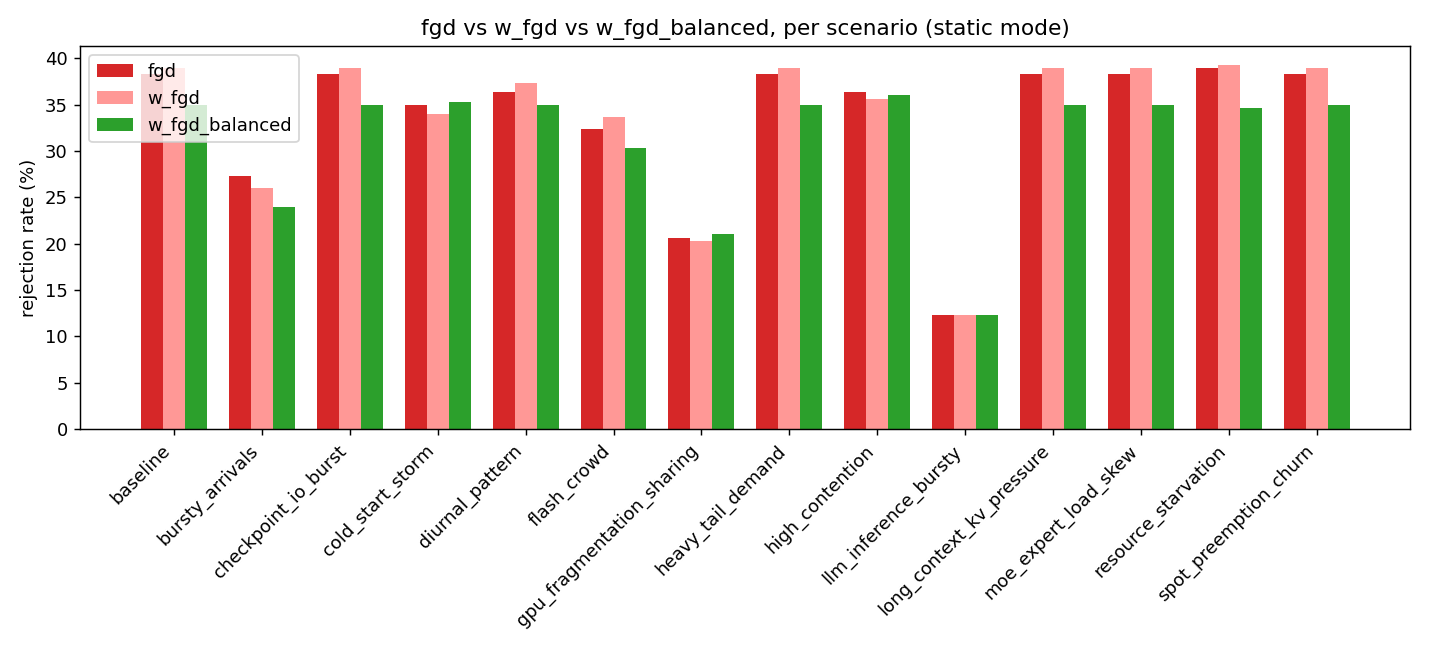
\includegraphics[width=0.9\textwidth]{plots/02_fgd_vs_wfgd_per_scenario.png}
\end{frame}

\begin{frame}{Broader Metrics: Beyond Rejection Rate}
\centering
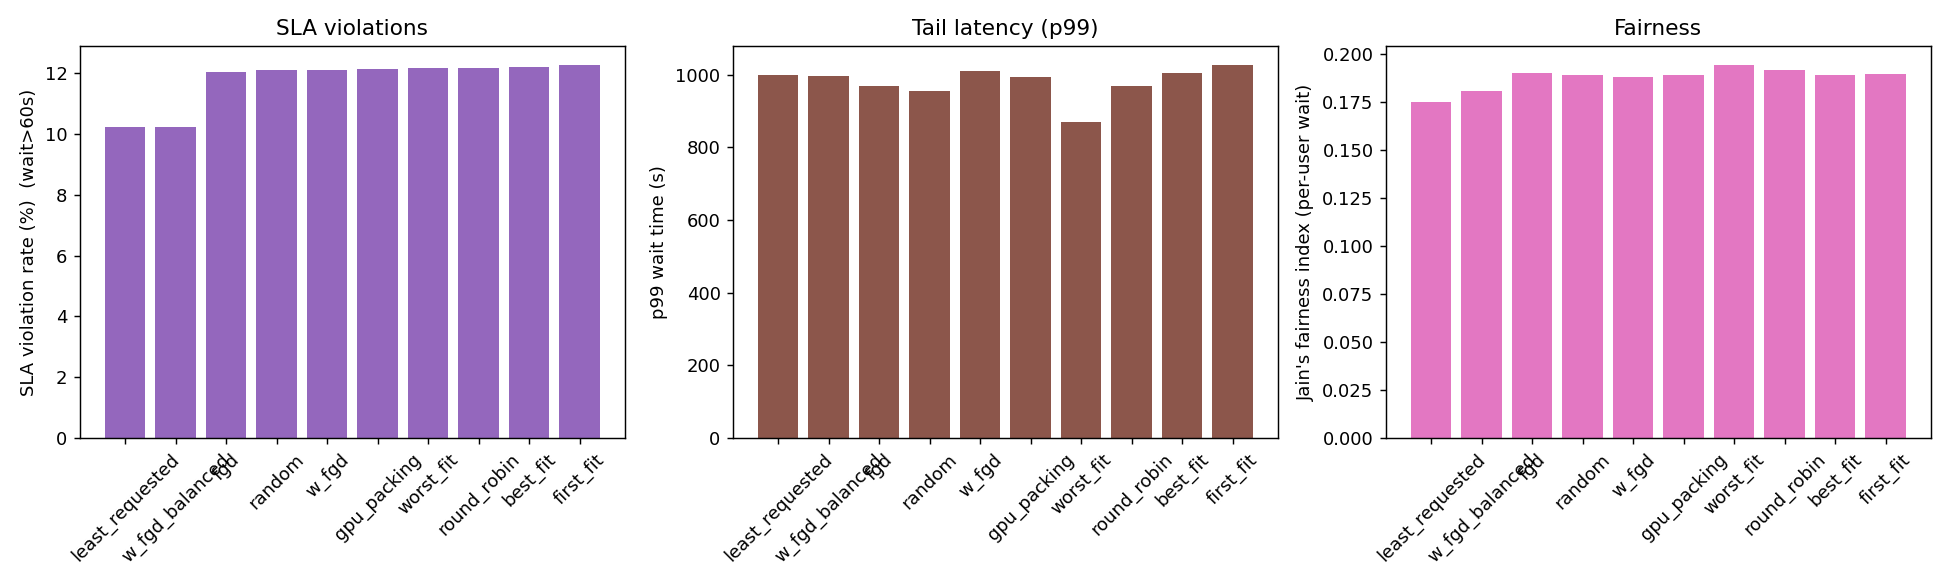
\includegraphics[width=\textwidth]{plots/03_broader_metrics_comparison.png}
\end{frame}

\begin{frame}{Scenario Difficulty}
\centering
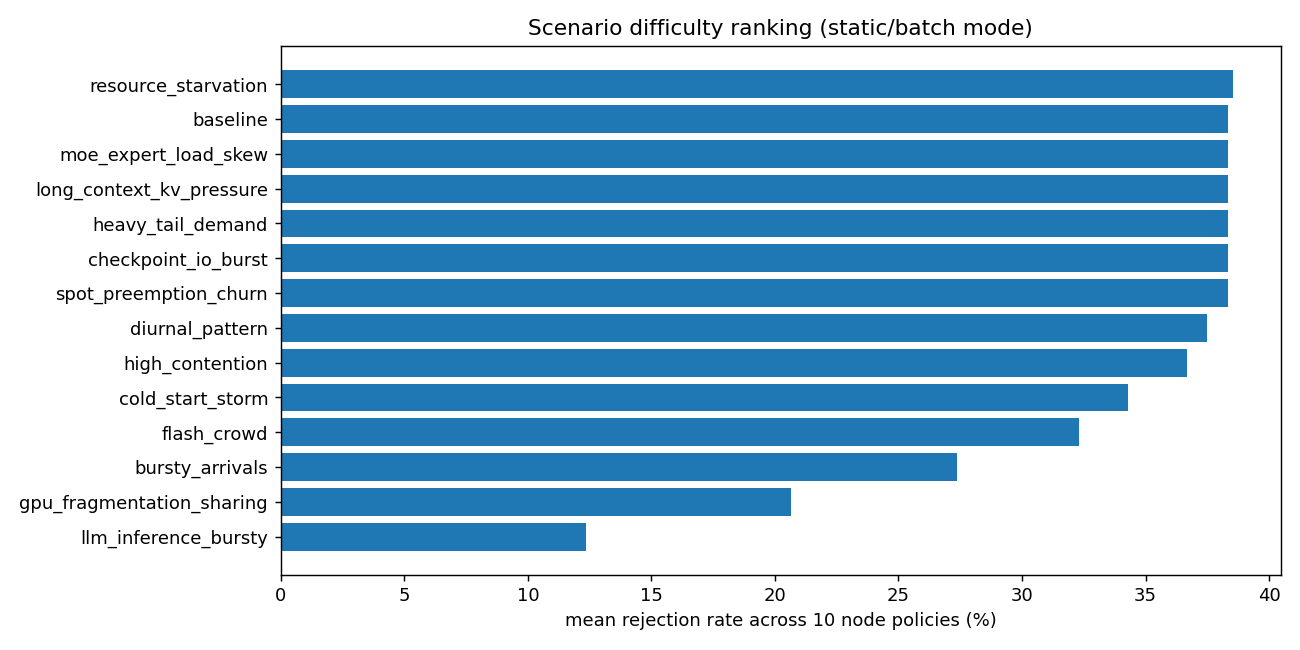
\includegraphics[width=0.75\textwidth]{plots/04_scenario_difficulty.png}
\end{frame}

\begin{frame}{An Honest Finding About Our Own Generator}
\small
\begin{tabular}{lcccc}
\toprule
scenario & GPU & CPU & duration & submit\_time \\
\midrule
\textbf{heavy\_tail\_demand} & \checkmark & \checkmark & \checkmark & \checkmark \\
checkpoint\_io\_burst & \checkmark & \checkmark & & \checkmark \\
high\_contention & \checkmark & \checkmark & \checkmark & \\
\bottomrule
\end{tabular}
\vspace{0.5cm}

\checkmark\ = identical to baseline, seed 42.

\begin{alertblock}{heavy\_tail\_demand is identical to baseline in \emph{every} column}
Its name describes a resource-size change that isn't happening in the
current generator -- we report this as a bug to fix, not hide it.
\end{alertblock}
\end{frame}

% =====================================================================
\section{Conclusion}
\begin{frame}{What We Actually Showed}
\begin{itemize}
  \item \textbf{Built} the missing stress-test instrument (gputrace,
    14 scenarios, statistically fit and individually justified)
  \item \textbf{Found} two specific, checkable weaknesses in FGD's metric
  \item \textbf{Fixed} them (w\_fgd, w\_fgd\_balanced) -- significant
    improvement over FGD, SLA violations
  \item \textbf{Reported honestly}: not better than the simplest existing
    baseline; found a real bug in our own generator; found and fixed a
    real performance bug in our own simulator
\end{itemize}
\vspace{0.4cm}
\centering
\alert{The null result is a finding: the field doesn't yet have a
benchmark broad enough to reliably tell real improvement from noise.}
\end{frame}

\begin{frame}{Future Directions}
\begin{enumerate}
  \item Sub-linear pending-queue structure (beyond our constant-factor fix)
  \item Learned $\lambda$, not grid-searched
  \item Disentangle H-TAFM's granularity vs.\ memory-assumption confounds
  \item Fix the heavy\_tail\_demand discrepancy upstream
  \item Scale to production-representative cluster and job counts
\end{enumerate}
\vspace{0.6cm}
\centering
\textbf{Everything reproduces from one archived checkpoint:}\\
\small \texttt{experiments/runs/2026-09-12\_fgd\_vs\_wfgd\_htafm/}
\end{frame}

\begin{frame}
\centering
\Huge Thank you
\vspace{0.5cm}

\normalsize\url{https://github.com/anuxlab/py_sim}\\
\url{https://github.com/anuxlab/simulated_data_generation_GPU_Scheduling}
\end{frame}

\end{document}
